% Created by tikzDevice version 0.12.3.1 on 2022-09-01 15:51:39
% !TEX encoding = UTF-8 Unicode
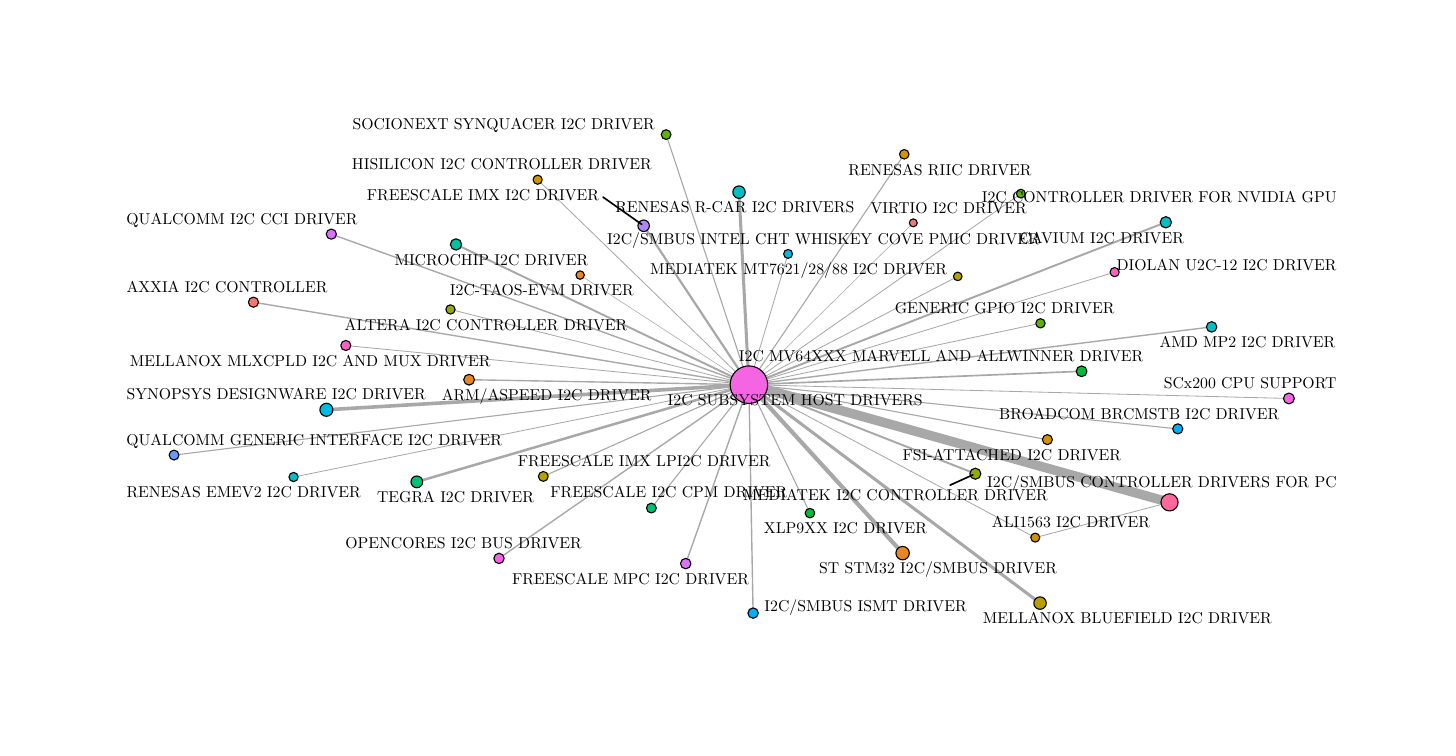
\begin{tikzpicture}[x=1pt,y=1pt]
\definecolor{fillColor}{RGB}{255,255,255}
\path[use as bounding box,fill=fillColor,fill opacity=0.00] (0,0) rectangle (505.89,252.94);
\begin{scope}
\path[clip] (  0.00,  0.00) rectangle (505.89,252.94);
\definecolor{fillColor}{RGB}{255,255,255}

\path[fill=fillColor] (  0.00,  0.00) rectangle (505.89,252.94);
\end{scope}
\begin{scope}
\path[clip] ( 32.75, 32.75) rectangle (475.89,222.94);
\definecolor{drawColor}{gray}{0.66}

\path[draw=drawColor,line width= 0.3pt,line join=round] (364.08, 68.68) -- (260.61,123.93);

\path[draw=drawColor,line width= 0.3pt,line join=round] (364.08, 68.68) -- (412.60, 81.41);

\path[draw=drawColor,line width= 0.3pt,line join=round] (152.78,151.12) -- (260.61,123.93);

\path[draw=drawColor,line width= 0.5pt,line join=round] (427.82,144.81) -- (260.61,123.93);

\path[draw=drawColor,line width= 0.5pt,line join=round] (159.50,125.73) -- (260.61,123.93);

\path[draw=drawColor,line width= 0.5pt,line join=round] ( 81.58,153.74) -- (260.61,123.93);

\path[draw=drawColor,line width= 0.4pt,line join=round] (415.59,107.97) -- (260.61,123.93);

\path[draw=drawColor,line width= 0.7pt,line join=round] (411.27,182.61) -- (260.61,123.93);

\path[draw=drawColor,line width= 0.3pt,line join=round] (392.77,164.60) -- (260.61,123.93);

\path[draw=drawColor,line width= 0.4pt,line join=round] (225.37, 79.35) -- (260.61,123.93);

\path[draw=drawColor,line width= 0.8pt,line join=round] (222.58,181.36) -- (260.61,123.93);

\path[draw=drawColor,line width= 0.4pt,line join=round] (186.32, 90.78) -- (260.61,123.93);

\path[draw=drawColor,line width= 0.5pt,line join=round] (237.78, 59.28) -- (260.61,123.93);

\path[draw=drawColor,line width= 0.4pt,line join=round] (368.47,104.08) -- (260.61,123.93);

\path[draw=drawColor,line width= 0.3pt,line join=round] (365.97,146.11) -- (260.61,123.93);

\path[draw=drawColor,line width= 0.3pt,line join=round] (184.27,198.01) -- (260.61,123.93);

\path[draw=drawColor,line width= 0.3pt,line join=round] (358.88,192.97) -- (260.61,123.93);

\path[draw=drawColor,line width= 0.6pt,line join=round] (380.83,128.77) -- (260.61,123.93);

\path[draw=drawColor,line width= 0.2pt,line join=round] (260.61,123.93) -- (199.63,163.54);

\path[draw=drawColor,line width= 3.4pt,line join=round] (260.61,123.93) -- (412.60, 81.41);

\path[draw=drawColor,line width= 0.3pt,line join=round] (260.61,123.93) -- (274.77,171.19);

\path[draw=drawColor,line width= 0.5pt,line join=round] (260.61,123.93) -- (262.13, 41.40);

\path[draw=drawColor,line width= 0.7pt,line join=round] (260.61,123.93) -- (342.44, 91.76);

\path[draw=drawColor,line width= 0.3pt,line join=round] (260.61,123.93) -- (336.08,163.06);

\path[draw=drawColor,line width= 1.1pt,line join=round] (260.61,123.93) -- (365.81, 45.01);

\path[draw=drawColor,line width= 0.3pt,line join=round] (260.61,123.93) -- (114.96,138.09);

\path[draw=drawColor,line width= 0.7pt,line join=round] (260.61,123.93) -- (154.79,174.61);

\path[draw=drawColor,line width= 0.5pt,line join=round] (260.61,123.93) -- (170.31, 61.16);

\path[draw=drawColor,line width= 0.4pt,line join=round] (260.61,123.93) -- ( 52.89, 98.50);

\path[draw=drawColor,line width= 0.5pt,line join=round] (260.61,123.93) -- (109.72,178.33);

\path[draw=drawColor,line width= 0.3pt,line join=round] (260.61,123.93) -- ( 96.08, 90.56);

\path[draw=drawColor,line width= 1.1pt,line join=round] (260.61,123.93) -- (257.04,193.51);

\path[draw=drawColor,line width= 0.4pt,line join=round] (260.61,123.93) -- (316.75,207.19);

\path[draw=drawColor,line width= 0.3pt,line join=round] (260.61,123.93) -- (455.75,118.95);

\path[draw=drawColor,line width= 0.4pt,line join=round] (260.61,123.93) -- (230.70,214.30);

\path[draw=drawColor,line width= 1.5pt,line join=round] (260.61,123.93) -- (316.16, 63.06);

\path[draw=drawColor,line width= 1.3pt,line join=round] (260.61,123.93) -- (107.94,114.86);

\path[draw=drawColor,line width= 0.9pt,line join=round] (260.61,123.93) -- (140.62, 88.82);

\path[draw=drawColor,line width= 0.2pt,line join=round] (260.61,123.93) -- (320.01,182.41);

\path[draw=drawColor,line width= 0.4pt,line join=round] (260.61,123.93) -- (282.67, 77.52);
\definecolor{drawColor}{RGB}{0,0,0}
\definecolor{fillColor}{RGB}{211,146,0}

\path[draw=drawColor,line width= 0.4pt,line join=round,line cap=round,fill=fillColor] (364.08, 68.68) circle (  1.63);
\definecolor{fillColor}{RGB}{147,170,0}

\path[draw=drawColor,line width= 0.4pt,line join=round,line cap=round,fill=fillColor] (152.78,151.12) circle (  1.68);
\definecolor{fillColor}{RGB}{0,191,196}

\path[draw=drawColor,line width= 0.4pt,line join=round,line cap=round,fill=fillColor] (427.82,144.81) circle (  1.89);
\definecolor{fillColor}{RGB}{232,133,38}

\path[draw=drawColor,line width= 0.4pt,line join=round,line cap=round,fill=fillColor] (159.50,125.73) circle (  1.95);
\definecolor{fillColor}{RGB}{248,118,109}

\path[draw=drawColor,line width= 0.4pt,line join=round,line cap=round,fill=fillColor] ( 81.58,153.74) circle (  1.83);
\definecolor{fillColor}{RGB}{0,173,250}

\path[draw=drawColor,line width= 0.4pt,line join=round,line cap=round,fill=fillColor] (415.59,107.97) circle (  1.83);
\definecolor{fillColor}{RGB}{0,191,196}

\path[draw=drawColor,line width= 0.4pt,line join=round,line cap=round,fill=fillColor] (411.27,182.61) circle (  2.04);
\definecolor{fillColor}{RGB}{255,97,195}

\path[draw=drawColor,line width= 0.4pt,line join=round,line cap=round,fill=fillColor] (392.77,164.60) circle (  1.66);
\definecolor{fillColor}{RGB}{0,191,116}

\path[draw=drawColor,line width= 0.4pt,line join=round,line cap=round,fill=fillColor] (225.37, 79.35) circle (  1.77);
\definecolor{fillColor}{RGB}{174,135,255}

\path[draw=drawColor,line width= 0.4pt,line join=round,line cap=round,fill=fillColor] (222.58,181.36) circle (  2.07);
\definecolor{fillColor}{RGB}{183,159,0}

\path[draw=drawColor,line width= 0.4pt,line join=round,line cap=round,fill=fillColor] (186.32, 90.78) circle (  1.78);
\definecolor{fillColor}{RGB}{219,114,251}

\path[draw=drawColor,line width= 0.4pt,line join=round,line cap=round,fill=fillColor] (237.78, 59.28) circle (  1.89);
\definecolor{fillColor}{RGB}{211,146,0}

\path[draw=drawColor,line width= 0.4pt,line join=round,line cap=round,fill=fillColor] (368.47,104.08) circle (  1.81);
\definecolor{fillColor}{RGB}{94,179,0}

\path[draw=drawColor,line width= 0.4pt,line join=round,line cap=round,fill=fillColor] (365.97,146.11) circle (  1.69);
\definecolor{fillColor}{RGB}{211,146,0}

\path[draw=drawColor,line width= 0.4pt,line join=round,line cap=round,fill=fillColor] (184.27,198.01) circle (  1.66);
\definecolor{fillColor}{RGB}{94,179,0}

\path[draw=drawColor,line width= 0.4pt,line join=round,line cap=round,fill=fillColor] (358.88,192.97) circle (  1.59);
\definecolor{fillColor}{RGB}{0,186,56}

\path[draw=drawColor,line width= 0.4pt,line join=round,line cap=round,fill=fillColor] (380.83,128.77) circle (  1.94);
\definecolor{fillColor}{RGB}{245,100,227}

\path[draw=drawColor,line width= 0.4pt,line join=round,line cap=round,fill=fillColor] (260.61,123.93) circle (  6.78);
\definecolor{fillColor}{RGB}{232,133,38}

\path[draw=drawColor,line width= 0.4pt,line join=round,line cap=round,fill=fillColor] (199.63,163.54) circle (  1.52);
\definecolor{fillColor}{RGB}{255,105,156}

\path[draw=drawColor,line width= 0.4pt,line join=round,line cap=round,fill=fillColor] (412.60, 81.41) circle (  3.10);
\definecolor{fillColor}{RGB}{0,185,227}

\path[draw=drawColor,line width= 0.4pt,line join=round,line cap=round,fill=fillColor] (274.77,171.19) circle (  1.61);
\definecolor{fillColor}{RGB}{0,173,250}

\path[draw=drawColor,line width= 0.4pt,line join=round,line cap=round,fill=fillColor] (262.13, 41.40) circle (  1.88);
\definecolor{fillColor}{RGB}{147,170,0}

\path[draw=drawColor,line width= 0.4pt,line join=round,line cap=round,fill=fillColor] (342.44, 91.76) circle (  2.00);
\definecolor{fillColor}{RGB}{183,159,0}

\path[draw=drawColor,line width= 0.4pt,line join=round,line cap=round,fill=fillColor] (336.08,163.06) circle (  1.55);

\path[draw=drawColor,line width= 0.4pt,line join=round,line cap=round,fill=fillColor] (365.81, 45.01) circle (  2.25);
\definecolor{fillColor}{RGB}{255,97,195}

\path[draw=drawColor,line width= 0.4pt,line join=round,line cap=round,fill=fillColor] (114.96,138.09) circle (  1.82);
\definecolor{fillColor}{RGB}{0,193,159}

\path[draw=drawColor,line width= 0.4pt,line join=round,line cap=round,fill=fillColor] (154.79,174.61) circle (  2.05);
\definecolor{fillColor}{RGB}{245,100,227}

\path[draw=drawColor,line width= 0.4pt,line join=round,line cap=round,fill=fillColor] (170.31, 61.16) circle (  1.87);
\definecolor{fillColor}{RGB}{97,156,255}

\path[draw=drawColor,line width= 0.4pt,line join=round,line cap=round,fill=fillColor] ( 52.89, 98.50) circle (  1.78);
\definecolor{fillColor}{RGB}{219,114,251}

\path[draw=drawColor,line width= 0.4pt,line join=round,line cap=round,fill=fillColor] (109.72,178.33) circle (  1.84);
\definecolor{fillColor}{RGB}{0,191,196}

\path[draw=drawColor,line width= 0.4pt,line join=round,line cap=round,fill=fillColor] ( 96.08, 90.56) circle (  1.66);

\path[draw=drawColor,line width= 0.4pt,line join=round,line cap=round,fill=fillColor] (257.04,193.51) circle (  2.24);
\definecolor{fillColor}{RGB}{211,146,0}

\path[draw=drawColor,line width= 0.4pt,line join=round,line cap=round,fill=fillColor] (316.75,207.19) circle (  1.72);
\definecolor{fillColor}{RGB}{245,100,227}

\path[draw=drawColor,line width= 0.4pt,line join=round,line cap=round,fill=fillColor] (455.75,118.95) circle (  1.97);
\definecolor{fillColor}{RGB}{94,179,0}

\path[draw=drawColor,line width= 0.4pt,line join=round,line cap=round,fill=fillColor] (230.70,214.30) circle (  1.76);
\definecolor{fillColor}{RGB}{232,133,38}

\path[draw=drawColor,line width= 0.4pt,line join=round,line cap=round,fill=fillColor] (316.16, 63.06) circle (  2.42);
\definecolor{fillColor}{RGB}{0,185,227}

\path[draw=drawColor,line width= 0.4pt,line join=round,line cap=round,fill=fillColor] (107.94,114.86) circle (  2.35);
\definecolor{fillColor}{RGB}{0,191,116}

\path[draw=drawColor,line width= 0.4pt,line join=round,line cap=round,fill=fillColor] (140.62, 88.82) circle (  2.12);
\definecolor{fillColor}{RGB}{248,118,109}

\path[draw=drawColor,line width= 0.4pt,line join=round,line cap=round,fill=fillColor] (320.01,182.41) circle (  1.43);
\definecolor{fillColor}{RGB}{0,186,56}

\path[draw=drawColor,line width= 0.4pt,line join=round,line cap=round,fill=fillColor] (282.67, 77.52) circle (  1.73);

\path[draw=drawColor,line width= 0.6pt,line join=round,line cap=round] (207.91,191.71) -- (221.92,181.83);

\path[draw=drawColor,line width= 0.6pt,line join=round,line cap=round] (333.32, 87.63) -- (341.56, 91.36);

\node[text=drawColor,anchor=base,inner sep=0pt, outer sep=0pt, scale=  0.57] at (376.99, 72.27) {ALI1563 I2C DRIVER};

\node[text=drawColor,anchor=base,inner sep=0pt, outer sep=0pt, scale=  0.57] at (165.62,143.64) {ALTERA I2C CONTROLLER DRIVER};

\node[text=drawColor,anchor=base,inner sep=0pt, outer sep=0pt, scale=  0.57] at (440.74,137.31) {AMD MP2 I2C DRIVER};

\node[text=drawColor,anchor=base,inner sep=0pt, outer sep=0pt, scale=  0.57] at (187.51,118.25) {ARM/ASPEED I2C DRIVER};

\node[text=drawColor,anchor=base,inner sep=0pt, outer sep=0pt, scale=  0.57] at ( 72.02,157.29) {AXXIA I2C CONTROLLER};

\node[text=drawColor,anchor=base,inner sep=0pt, outer sep=0pt, scale=  0.57] at (401.66,111.52) {BROADCOM BRCMSTB I2C DRIVER};

\node[text=drawColor,anchor=base,inner sep=0pt, outer sep=0pt, scale=  0.57] at (388.12,175.13) {CAVIUM I2C DRIVER};

\node[text=drawColor,anchor=base,inner sep=0pt, outer sep=0pt, scale=  0.57] at (433.21,165.19) {DIOLAN U2C-12 I2C DRIVER};

\node[text=drawColor,anchor=base,inner sep=0pt, outer sep=0pt, scale=  0.57] at (231.66, 83.31) {FREESCALE I2C CPM DRIVER};

\node[text=drawColor,anchor=base,inner sep=0pt, outer sep=0pt, scale=  0.57] at (164.52,190.53) {FREESCALE IMX I2C DRIVER};

\node[text=drawColor,anchor=base,inner sep=0pt, outer sep=0pt, scale=  0.57] at (222.77, 94.33) {FREESCALE IMX LPI2C DRIVER};

\node[text=drawColor,anchor=base,inner sep=0pt, outer sep=0pt, scale=  0.57] at (217.82, 51.82) {FREESCALE MPC I2C DRIVER};

\node[text=drawColor,anchor=base,inner sep=0pt, outer sep=0pt, scale=  0.57] at (355.63, 96.61) {FSI-ATTACHED I2C DRIVER};

\node[text=drawColor,anchor=base,inner sep=0pt, outer sep=0pt, scale=  0.57] at (353.04,149.70) {GENERIC GPIO I2C DRIVER};

\node[text=drawColor,anchor=base,inner sep=0pt, outer sep=0pt, scale=  0.57] at (171.34,201.59) {HISILICON I2C CONTROLLER DRIVER};

\node[text=drawColor,anchor=base,inner sep=0pt, outer sep=0pt, scale=  0.57] at (408.89,189.75) {I2C CONTROLLER DRIVER FOR NVIDIA GPU};

\node[text=drawColor,anchor=base,inner sep=0pt, outer sep=0pt, scale=  0.57] at (330.06,132.32) {I2C MV64XXX MARVELL AND ALLWINNER DRIVER};

\node[text=drawColor,anchor=base,inner sep=0pt, outer sep=0pt, scale=  0.57] at (277.34,116.46) {I2C SUBSYSTEM HOST DRIVERS};

\node[text=drawColor,anchor=base,inner sep=0pt, outer sep=0pt, scale=  0.57] at (185.81,156.04) {I2C-TAOS-EVM DRIVER};

\node[text=drawColor,anchor=base,inner sep=0pt, outer sep=0pt, scale=  0.57] at (409.86, 86.63) {I2C/SMBUS CONTROLLER DRIVERS FOR PC};

\node[text=drawColor,anchor=base,inner sep=0pt, outer sep=0pt, scale=  0.57] at (287.56,174.75) {I2C/SMBUS INTEL CHT WHISKEY COVE PMIC DRIVER};

\node[text=drawColor,anchor=base,inner sep=0pt, outer sep=0pt, scale=  0.57] at (302.77, 41.85) {I2C/SMBUS ISMT DRIVER};

\node[text=drawColor,anchor=base,inner sep=0pt, outer sep=0pt, scale=  0.57] at (313.56, 82.21) {MEDIATEK I2C CONTROLLER DRIVER};

\node[text=drawColor,anchor=base,inner sep=0pt, outer sep=0pt, scale=  0.57] at (278.54,163.66) {MEDIATEK MT7621/28/88 I2C DRIVER};

\node[text=drawColor,anchor=base,inner sep=0pt, outer sep=0pt, scale=  0.57] at (397.37, 37.53) {MELLANOX BLUEFIELD I2C DRIVER};

\node[text=drawColor,anchor=base,inner sep=0pt, outer sep=0pt, scale=  0.57] at (102.08,130.59) {MELLANOX MLXCPLD I2C AND MUX DRIVER};

\node[text=drawColor,anchor=base,inner sep=0pt, outer sep=0pt, scale=  0.57] at (167.57,167.16) {MICROCHIP I2C DRIVER};

\node[text=drawColor,anchor=base,inner sep=0pt, outer sep=0pt, scale=  0.57] at (157.51, 64.70) {OPENCORES I2C BUS DRIVER};

\node[text=drawColor,anchor=base,inner sep=0pt, outer sep=0pt, scale=  0.57] at (103.50,102.04) {QUALCOMM GENERIC INTERFACE I2C DRIVER};

\node[text=drawColor,anchor=base,inner sep=0pt, outer sep=0pt, scale=  0.57] at ( 77.45,181.89) {QUALCOMM I2C CCI DRIVER};

\node[text=drawColor,anchor=base,inner sep=0pt, outer sep=0pt, scale=  0.57] at ( 78.03, 83.07) {RENESAS EMEV2 I2C DRIVER};

\node[text=drawColor,anchor=base,inner sep=0pt, outer sep=0pt, scale=  0.57] at (255.52,185.99) {RENESAS R-CAR I2C DRIVERS};

\node[text=drawColor,anchor=base,inner sep=0pt, outer sep=0pt, scale=  0.57] at (329.66,199.68) {RENESAS RIIC DRIVER};

\node[text=drawColor,anchor=base,inner sep=0pt, outer sep=0pt, scale=  0.57] at (441.74,122.52) {SCx200 CPU SUPPORT};

\node[text=drawColor,anchor=base,inner sep=0pt, outer sep=0pt, scale=  0.57] at (171.98,216.01) {SOCIONEXT SYNQUACER I2C DRIVER};

\node[text=drawColor,anchor=base,inner sep=0pt, outer sep=0pt, scale=  0.57] at (328.95, 55.60) {ST STM32 I2C/SMBUS DRIVER};

\node[text=drawColor,anchor=base,inner sep=0pt, outer sep=0pt, scale=  0.57] at ( 89.78,118.42) {SYNOPSYS DESIGNWARE I2C DRIVER};

\node[text=drawColor,anchor=base,inner sep=0pt, outer sep=0pt, scale=  0.57] at (154.61, 81.33) {TEGRA I2C DRIVER};

\node[text=drawColor,anchor=base,inner sep=0pt, outer sep=0pt, scale=  0.57] at (332.78,185.96) {VIRTIO I2C DRIVER};

\node[text=drawColor,anchor=base,inner sep=0pt, outer sep=0pt, scale=  0.57] at (295.50, 70.04) {XLP9XX I2C DRIVER};
\end{scope}
\end{tikzpicture}
